

\subsection{Sensor Calibration}

A planar checkerboard pattern was used to calibrate all three cameras to obtain both intrinsic and extrinsic parameters.  While the grid pattern is not visible in the depth image, it is nevertheless observed in the reflected IR image whose pixels correspond to the depth pixels.  This enables the use of Zhang's method~\cite{Zhang2000} to calculate the intrinsic parameters including a $2$-parameter radial distortion of each camera.  In this process the poses of all three cameras are also calculated relative to the checkerboard.  The intrinsic and extrinsic parameters are stored as text files, and a Matlab function is provided that reads the parameters and can plot the camera poses as in Figure~\ref{fig:CameraConfiguration}.


\subsubsection{Noise Characterization}
\label{sec:bias}

The time of flight depth measurements can have significant noise, and it is useful to both model it and quantify it.  Doing so can lead to strategies to reduce noise as well as providing guidance to algorithms that use the depth measurements.  Our goal in this section is to provide a simple noise model that can predict the empirically observed depth noise on smooth, Lambertian surfaces, such as plant leafs.

The depth noise $\epsilon$ is modeled as the sum of two components, $\epsilon_I$ and $\epsilon_S$:
\begin{equation}
	\epsilon = \epsilon_I + \epsilon_S\label{eq:epsilon}
\end{equation}
The term $\epsilon_I$ captures the noise component that varies between images taken from a fixed pose of a static scene. On the other hand the term $\epsilon_S$ models noise that is constant between images but varies between pixels. The variance of $\epsilon_I$ can be estimated by observing pixels of a fixed scene over multiple images.  In our experiments we observed a flat, uniform albedo surface perpendicular to the camera at a sequence of depths, and for each depth acquiring 300 images.  Object depth has a large impact on $\epsilon_I$ likely due to reduced reflected signal.  For constant depth, we observed that the primary factor affecting the variance is the pixel radius from the image center.  Physically we expect this dependence is due to a circularly symmetric illuminating beam closely aligned with the optical axis.  Based on these observations $\sigma_I^2$, the variance of $\epsilon_I$, is empirically estimated as a function of object depth and pixel radius as shown in Figure~\ref{fig:Noise}.

\begin{table*}[t!]
\begin{center}
\caption{Summary of Arabidopsis and Bean databases.}
\label{tab:stat}
\begin{tabular}{c|c|c|c|c|c}
      \hline
      % after \\: \hline or \cline{col1-col2} \cline{col3-col4} ...
      Plants     & Subjects & Days & Images/Day & Total Images & Annotated Images \\
      \hline
      Arabidopsis &  $16$      &  $9$   &     $16$     &     $2304\times 4$     &       $576\times 4$     \\
      \hline
      Bean        &   $5$      &  $5$   &     $14$     &     $350\times 4$       &       $175\times 4$  \\
      \hline
\end{tabular}
\end{center}
\end{table*}



\begin{table*}
\begin{center}
\caption{Plant image resolution of Arabidopsis and Bean databases.}
\label{tab:resolution}
\begin{tabular}{c|c|c|c|c}
      \hline
      % after \\: \hline or \cline{col1-col2} \cline{col3-col4} ...
      Plants     & Fluorescence       & IR        & RGB      & Depth     \\
      \hline
      Arabidopsis &  $\sim$$240\times240$ &  $\sim$$240\times240$  & $\sim$$120\times120$  & $\sim$$25\times25$  \\
      %\hline
      Bean        & $1000\times640$ & $1000\times640$ & $380\times720$ & $90\times190$    \\
      \hline
\end{tabular}
\end{center}
\end{table*}

In addition to image-varying noise, there are pixel depth offsets that are constant for images of the same scene so cannot be removed by averaging over many frames.  We model these with $\epsilon_S$.  To estimate its variance, $\sigma_S^2$, we first average over many depth measurement images, in our case 300, to obtain pixel depth estimates that approximately eliminate the effect of $\epsilon_I$.  Then by calculating true ray depths on a known surface, in our case the observed plane, and assuming that $\epsilon_S$ has the same distribution over all pixels, $\sigma_S^2$ is obtained as the variance of the error between averaged depths and known depths.  In our experiments we obtained $\sigma_S=6.5mm$, and found that it was insensitive to changes in depth.



Assuming independence of $\epsilon_I$ and $\epsilon_S$, the expected variance of depth measurements in the data collection can be obtained as follows.  When $N$ images are averaged to obtain a depth image, where $N=5$ for our data collection, the depth variance is predicted to be:
\begin{equation}
	\sigma^2 = \frac{\sigma_I^2}{N} + \sigma_S^2.\label{eq:sigma}
\end{equation}

There are additional sources of noise not captured by this including object specularities, sharp variations in object albedo, mixed-depth pixels on object edges, and cases of very-low signal reflection.  In addition we noticed that the chamber light shades blocked some of the depth camera field of view, and in doing so reflected some of the IR illumination.  This resulted in a small constant depth shift for the pixels.  We measured this shift for each chamber experiment and provide it as an optional correction to the depth images.

%\begin{figure}
%\begin{centering}
%\begin{tabular}{c }
%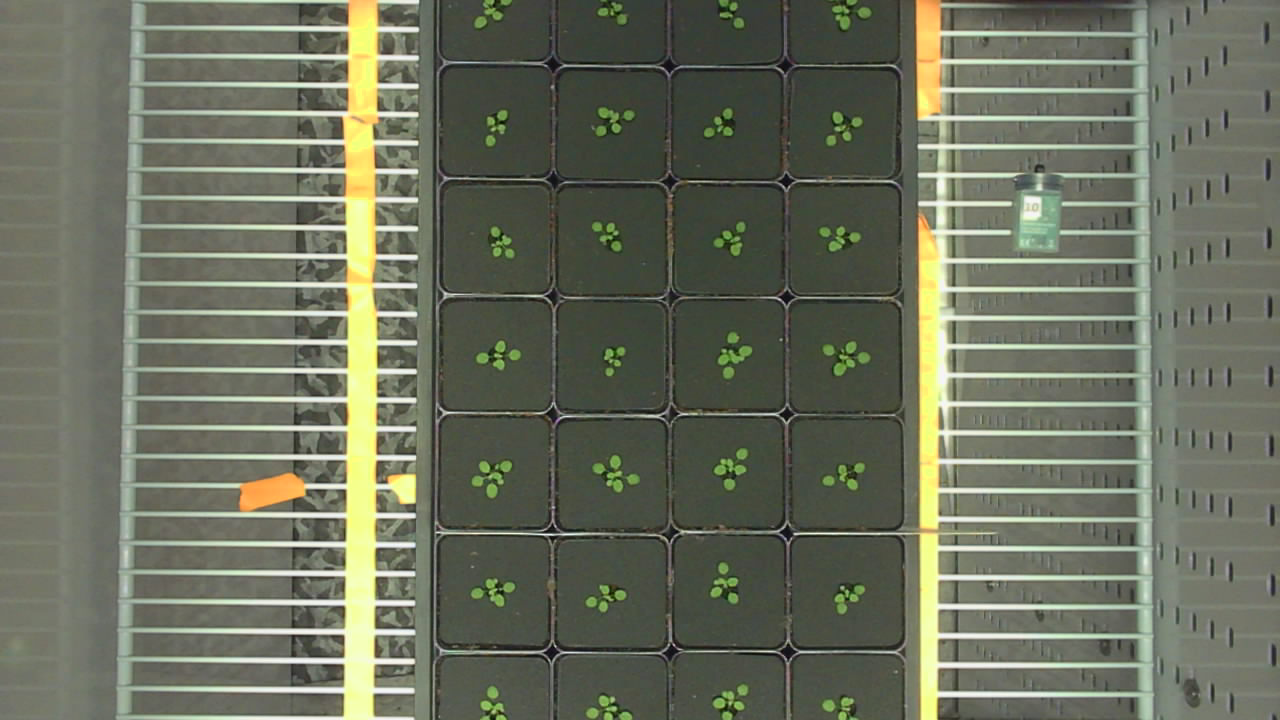
\includegraphics[width=.47\textwidth]{Figures/rawImages/a.png}\\
%Arabidopsis \\
%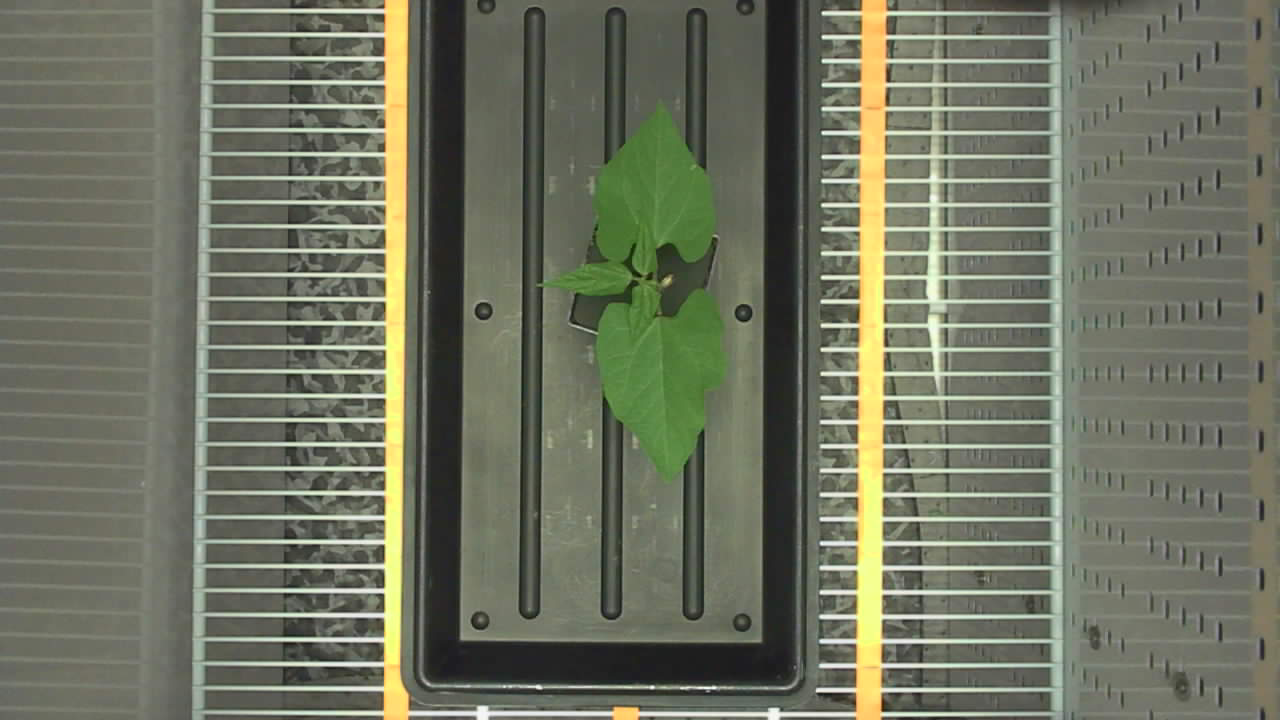
\includegraphics[width=.47\textwidth]{Figures/rawImages/b.png}\\
%   Bean \\
%\end{tabular}
%\caption{RGB color images of Arabidopsis and bean plants. }
%\label{fig:rawIm}
%\end{centering}
%\end{figure}



